% Taken verbatim from comps Q7

% A pitch-spelling algorithm is an algorithm that attempts
% to recreate the original spelling of a pitch-class in the
% context of a musical composition.

% This is a common problem in MIDI representations, as MIDI
% representations \emph{drop} all the spelling information
% of a note, leaving only the pitch class and octave.

% However, this is not an exclusive problem associated with
% MIDI representations, it would also happen when we observe
% the performance of a piece in a piano keyboard, we do not
% explicitly know whether the key played by the performer
% was intended to be an F\# or a Gb.

% Different approaches have been attempted to reconstruct
% the original spelling of a musical score.

% One of the advantages of pitch-spelling as a computational
% problem, is that it is much easier to evaluate than other
% musical problems like key classification or chord
% recognition, as it presents less ambiguity.

% \guide{Meredith}



% Meredith and Wiggins suggest that pitch-spelling
% algorithms can be used to improve the performance of
% key-finding algorithms.

% The study of Meredith and Wiggins is limited to music from
% the baroque and classical period. As of now, there are
% high-quality corpora of 19th century romantic music that
% could be integrated in a similar study.

% Meredith and Wiggins suggest that until no reliable
% pitch-spelling algorithm exists, it is theoretically
% impossible to reconstruct a notated score if given only a
% MIDI file as input.

% According to Meredith and Wiggins, knowing the spelling of
% a name also facilitates certain type of musical queries,
% for example, looking for a sequence of diatonic intervals.
% Without the knowledge of the spelling, these type of
% queries can only be approximated, and according to their
% research, they are also slower than looking for an exact
% match.

% In the study by Meredith and Wiggins, the evaluation
% metric is the raw proportion of note names that have been
% correctly spelled from the total number of spellings in
% the dataset. It is important to remark that the spellings
% of notes are not evenly distributed, particularly for
% diatonic degrees of the C Major scale (i.e., white keys in
% a piano keyboard). That is, an algorithm that predicts the
% pitch-class 0 as C would be correct most of the times, as
% it is rarely spelled as B\# or Dbb. In machine learning
% classification experiments, this problem is usually
% addressed by using different metrics of evaluation that
% account for a sparse distribution of the classes in the
% dataset. The problem of pitch-spelling requires,
% therefore, an improved method of evaluation that provides
% more meaningful information than the raw number of notes
% that have been correctly spelled.

% A derivate issue of pitch spelling algorithms is---what I
% denote---an accidental overflow. When the tonal changes in
% a score lead to a key that requires an exhaustive use of
% accidentals (e.g., double flats, or double sharps),
% composers will likely move the spellings to have less
% accidentals, for example, by notating the music in an
% enharmonic key instead.

% Meredith and Wiggins discuss one instance of such
% accidental overflow that they found in their dataset,
% Haydn's Symphony No. 100 in G Major ('Military'), in which
% a sudden change of pitch spellings implies that the piece
% moved from Db Major to C# Major, although the only
% motivation of this change of spelling is to simplify the
% notation.

% Meredith and Wiggins address this issue in their
% evaluation by providing alternative assessments of that
% fragment of music, that is, if an algorithm decided to
% spell the entire section as either C# Major, Db Major, or
% change it midways, they should all be considered correct
% to a certain extent. This, of course, is one instance of
% such issue but it needs to be addressed more formally in
% future evaluations.

% Meredith and Wiggins provide a review of 5 pitch-spelling
% algorithms (plus several variations of those algorithms):
% Longuet-Higgins, Cambouropoulos, Temperley and Sleator,
% Chew and Chen, and Meredith.

% In the evaluation from Meredith and Wiggins, the inclusion
% of sections with accidental overflow reduced the accuracy
% score of the algorithms, particularly, Temperley and
% Sleator, to the point that this section was removed from
% the evaluation.

% \guide{teodoru and raphael} Teodoru and Raphael presented
% a pitch-spelling algorithm that was tested using the same
% dataset used previously by Meredith. Their algorithm
% performs favorably compared to the other known
% pitch-spelling algorithms.

% Teodoru and Raphael note the necessity of a reliable
% pitch-spelling algorithm, particularly for the use within
% music notation software. They note: "[...] at present, the
% pitch-spellings from the commercial music notation
% programs we know of leave much to be desired". It is worth
% mentioning that over a decade has passed since this paper
% was published and researching the current state of
% pitch-spelling algorithms implemented in commercial music
% notation software could show substantial improvement
% today.

% Teodoru and Raphael tackle the problem by assuming that
% the spelling of a note can be explained through analyzing
% voice leading and local harmony.

% Teodoru and Raphael collect principles and guidelines for
% spelling notes from music theory textbooks, and try to
% incorporate such principles in the design of their
% algorithm. An example of those principles is taken from
% Aldwell's book: "avoiding “remote” accidentals; thus B♭ is
% preferred to A♯ in C major, since the former is in the
% scale of the F major, which is near to C.".

% It could be understood from such principles that there is
% an "optimal" spelling. Considering that the objective of
% spelling is to reduce the number of accidentals to the
% minimum, every spelling that is closer to C Major is
% therefore simpler, as it requires less accidentals in its
% spelling.

% Teodoru and Raphael claim that their algorithm produces an
% error that is lower than the best of Meredith's algorithms
% by a factor of more than 3.

% The model from Teodoru and Raphael assumes that the music
% will be provided as individual voices, which is a
% reasonable assumption for inputs that imply a separation
% of individual voices (i.e., chorales), but becomes a huge
% limitation for other keyboard music and other types of
% music where this separation is not provided and not
% obvious.

% Teodoru and Raphael claim that estimating the time-varying
% key (local key) is the most important element for pitch
% spelling. Additionally, they consider that the
% relationship between local keys and spelling is
% bidirectional, that is, spelling can help influence the
% choice of key as much as the key can influence the choice
% of spelling.

% Teodoru and Raphael replicate a study using the dataset
% derived by Meredith, however, the evaluation score is
% presented as an error rate, which consists in the number
% of misspelled notes divided by the total number of notes.
% They computed the error rate overall as well as for each
% of the composers in the dataset.

% Teodoru and Raphael describe that a subset of the corpus
% was used as "training data". The training data consisted
% of all of the Beethoven scores, 5 string quartet movements
% from Haydn, and a concerto movement from Mozart. This, of
% course, means that the performance shown in the paper does
% not contemplate the performance of the algorithm in a set
% of previously unseen data.

% Teodoru and Raphael report that their algorithm was
% particularly unable to correctly spell the pitches during
% harmonic progressions that involved German Augmented Sixth
% Chords, Diminished Seventh chords and other harmonic
% circumstances. They note: "Other situations require a
% deeper notion of the harmonic state than provided by the
% local key, as in the German augmented sixth chord, which
% seems nearly impossible to spell correctly without
% recognizing it as such." It may be possible that spelling
% the notes requires not only to model the interaction
% between keys and spelling but also of chords.

A pitch-spelling model is an algorithm that predicts the
original spelling that a note had in a musical score when
only the pitch-class, octave, and duration of the note are
provided as inputs to the model.\footnote{Some researchers
have also found helpful to know the voice (\emph{stream}, in
psychoacoustics) in which the note is sounding. However,
this information departs from what can be reliably obtained
from real-world digital music files. Therefore, a real-world
algorithm should work regardless of whether it knows what
voice played the note.}

To understand the problems that derive from pitch-spelling,
the following example could be considered. If during a
musical performance, a pianist presses the key corresponding
to the pitch class number 8 in the piano keyboard (shown in
Figure  \ref{fig:Q7_1}), how can we know if the note played
by the performer was an A$\flat$ or a
G$\sharp$?\footnote{Assume an equal-tempered setting, with
no special considerations regarding how the piano might be
tuned. That is, the distinction between the A$\flat$ and
G$\sharp$ notes that we are looking for is of a semantic
nature.}

% \begin{figure}[h] \centering
%     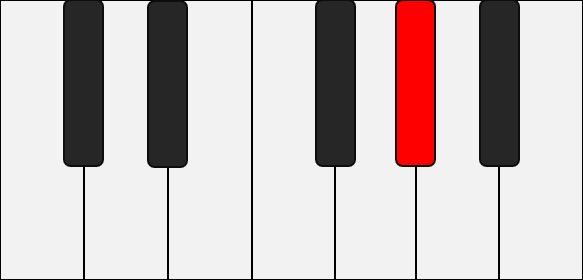
\includegraphics[width=0.6\textwidth]{figures/Q7_1.png}
%     \caption{A note playing in a keyboard. It could be
%     either G$\sharp$ or A$\flat$.} \label{fig:Q7_1}
%     \end{figure}

This example problem may seem ingenuous at first, however,
the spelling of a note could \emph{carry} much more
information about the tonal context of the music that one
might expect. Similarly, the reverse problem (spelling the
note) may \emph{require} much more information about the
tonal context of the music that one might expect. This
double relationship between the acquired and delivered
musical knowledge in the spelling of a note is what makes it
an interesting computational problem, as it provides a
framework for assessing quantitatively the extent to which a
computational model understands the musical semantics.
Furthermore, finding the spelling of a note has the
additional advantage of being highly unambiguous as an
evaluation metric compared to other analytical tasks like
finding the musical key \parencite{gebhardt2018confidence}
or labeling the chords in a piece
\parencite{ni2013understanding}.

In order to better contextualize what is the information
contained in the spelling of a pitch, let us extend the
previous thought exercise a bit further.

A first impulse that someone might have for guessing whether
the note is A$\flat$ or G$\sharp$ could be to know the
musical key of the piece during which the piano key was
played. Such information can be obtained from a key-finding
model and there are many approaches that could provide it
with a reasonable degree of accuracy. Nevertheless, our
pitch-spelling model now requires information about the key
in order to make its predictions.

It could be assumed that the model will receive such
predictions, and that they are reliable. A key-finding model
could then inform us that the piece was in \emph{A minor}.
``Is it a piece in A minor?'' Then the note is probably a
G$\sharp$.

% \begin{figure}[h] \centering
%     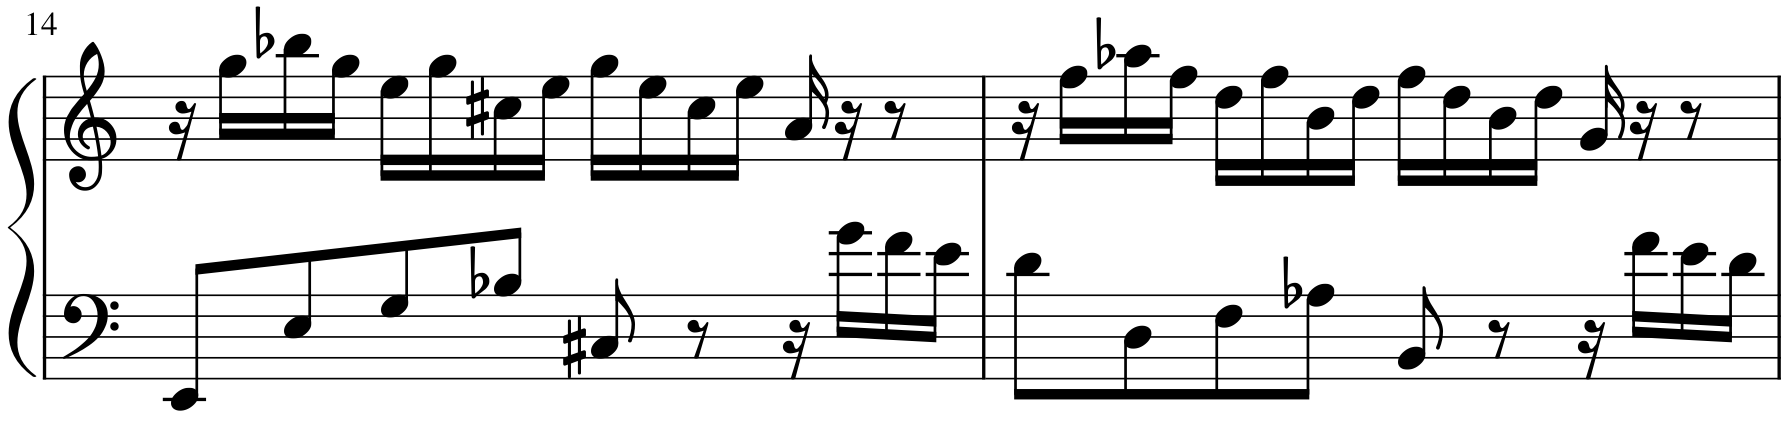
\includegraphics[width=0.8\textwidth]{figures/Q7_2.png}
%     \caption{J. S. Bach's BWV 784, mm. 14-15. The piece is
%     in A minor, however, during measure 15, the pitch
%     class number 8 is spelled as an A$\flat$.}
%     \label{fig:Q7_2} \end{figure}

Figure \ref{fig:Q7_2} shows an adversarial example where the
pitch class number 8 is spelled as A$\flat$ in a piece that
is originally in \emph{A minor}. A person familiarized with
Western tonal music could guess that similar examples as the
one shown in Figure \ref{fig:Q7_2} will occur whenever the
music is modulating or tonicizing a different key.

Assuming that the awareness of modulations and tonicizations
throughout the piece (which we generally refer to as
\emph{local keys}) will mitigate our problems when
predicting the spelling of a note, seems to be a reasonable
guess. Instead of requiring to know the \emph{global key} of
the piece, now, our model requires to know the \emph{local
keys} throughout the piece. Notice, however, that there are
much less models available that provide such information,
and that there is no sufficient amount of research assessing
whether they are accurate or not, mostly because the
concepts of modulation and tonicization are problematic and
ambiguous themselves (see Question \ref{chap:chap6} for a
further discussion on modulation and tonicization).

To complicate the matter a bit further, there are other
circumstances that affect the spelling of a note, such as
the use of non-chord tones or the harmonic context. One
example of the implications of non-chord tones is, as shown
in Figure \ref{fig:Q7_3}, the spelling of a chromatic
neighbouring note, which should probably have a different
note name than the \emph{real} note.

% \begin{figure}[h] \centering
%     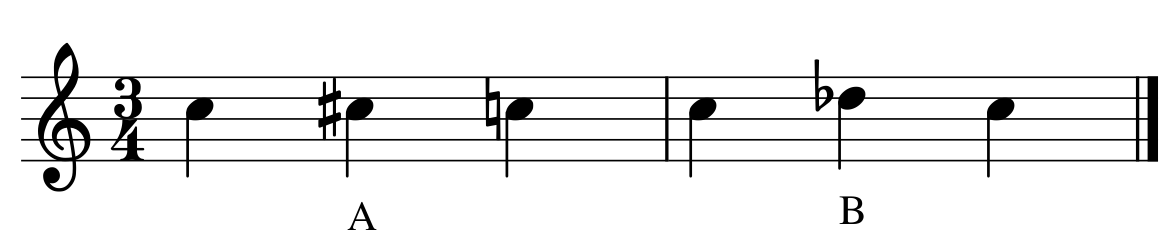
\includegraphics[width=0.8\textwidth]{figures/Q7_3.png}
%     \caption{Two notations (A and B) of a chromatic
%     neighbouring note. Regardless of the harmonic and key
%     context, the second note should probably be spelled as
%     in version B.} \label{fig:Q7_3} \end{figure}

One example of a complicated harmonic context is the
presence of a German augmented sixth, for which Teodoru and
Raphael write \parencite{teodoru2007pitch}: \emph{Other
situations require a deeper notion of the harmonic state
than provided by the local key, as in the German augmented
sixth chord, which seems nearly impossible to spell
correctly without recognizing it as such.}

Overall, designing a pitch-spelling algorithm poses
important challenges in different musical fronts, but it
also provides researchers with the opportunity of putting in
practice different analytical models (e.g., local key, chord
labeling, and non-chord detection) for solving a common
task. Furthermore, unlike many of those models which suffer
from highly ambiguous evaluations, pitch spelling presents a
simple way of assessing whether our computational models
understand the musical context or not. That is, the note is
either G$\sharp$ or A$\flat$, and there is only one right
answer.

In the following section, a survey is provided with
different pitch-spelling algorithms that have been developed
throughout the years.

\guide{A brief survey of pitch-spelling algorithms}

Compared to other tasks of Music Information Retrieval
(MIR), there have not been as many attempts to solve the
problem of pitch spelling. Nevertheless, it is likely that
there are other solutions to the problem, in commercial
applications, which are not described in the literature and
in this survey. This is due to the fact that pitch-spelling
is a highly relevant problem for commercial software that
deals with the conversion of MIDI files into music scores,
for example, most music notation editors.

% \guide{Longuet-Higgins (1976)}
In 1976, Longuet-Higgins presented what is arguably the
first pitch-spelling algorithm
\parencite{longuethiggins1976perception}. It is limited to
work on monophonic melodies. Longuet-Higgins considered that
any note could be assigned a number, $p$, based on
3-variables that related the note with respect to
\emph{middle C}: the distance in perfect fifths, the
distance in major thirds, and the octave. Using that
methodology, Longuet-Higgins extended the notation to add a
``sharpness'' feature, $q$, which was defined based on the
distance in fifths and thirds to \emph{middle C}, irrelevant
of the octave. This ``sharpness'' value, in conjunction with
the MIDI note number, was used to indicate the spelling of
the note.

% \guide{Cambouropoulos (2003)}
After a gap of around 25 years, a series of new algorithms
were developed by different researchers independently,
almost at the same time. In 2003, Cambouropoulos presents an
approach that heavily relies in intervals
\parencite{cambouropoulos2003pitch}. The algorithm uses a
shifting overlapping window (suggested to be of 9 to 12
pitches long). The window moves along the sequence of
pitches, from left to right, until the sequence concludes.
For each window, the pitch-spelling process optimizes two
aspects: 1) that notes make the minimum use of accidentals
(something that Cambouropoulos refers to as \emph{notational
parsimony}), and 2) the avoidance of 8 classes of augmented
and diminished intervals (something that Cambouropoulos
refers as \emph{interval optimization}). The algorithm was
evaluated on Mozart piano sonatas and Chopin Waltzes.

% \guide{Chew and Chen (2003)}
After its introduction in her dissertation, the Spiral Array
model by Chew was used for multiple tasks that involved
tonal analysis, for example, chord labeling, key-finding,
and pitch-spelling \parencite{chew2000towards}. The Spiral
Array is a spatial representation of tonality that allows a
sequence of pitches to be \emph{positioned} in
the---theoretical---tonal space, which facilitates the
computation of tonal features in different ways. Regarding
the pitch-spelling problem, three different algorithms were
proposed by Chew and Chen \parencite{chew2003determining}
that were built on top of each other. In the paper, their
evaluation of the algorithms restricted to few movements of
Beethoven's piano sonatas.

% \guide{Temperley and Sleator (2004)}
Throughout the late 1990s and early 2000s, Temperley
developed a series of algorithms for modelling different
aspects of musical structure (i.e., meter, phrasing,
counterpoint, harmony, key, and pitch-spelling). These
models were implemented by Daniel Sleator in the
\emph{Melisma Music Analyzer} and explained in detail in the
book by Temperley \parencite{temperley2004cognition}.
Respecting the pitch-spelling problem, the approach by
Temperley consists of a rule-based system based on his
concepts of \emph{Tonal Pitch Class (TPC)} and the
\emph{line of fifths}. Additionally, the algorithm depends
on the metrical analysis provided by the Melisma Music
Analyzer, before extracting the spelling of the notes.

% \guide{Meredith (2003)}
Meredith introduced an algorithm that receives MIDI note
numbers and onset times as ordered pairs and determines the
spelling of the notes through 2 stages
\parencite{meredith2003pitch}. The first stage consists of a
rule-based system with 8 rules that are carried out in
sequence. After the first stage, the algorithm has
determined a spelling for the notes. The second stage,
consists of the correction of the outputs given by the first
stage. The corrections performed account for neighbouring
notes or passing notes which could have been erroneously
predicted by the first stage. In a subsequent study
\parencite{meredith2005comparing}, Meredith compared its
pitch-spelling algorithm against other pitch spelling
algorithms, determining that his algorithm had the highest
accuracy.



% \guide{Stoddard et al. (2004)}
Stoddard et al. proposed a new algorithm for pitch-spelling
\parencite{stoddard2004welltempered}. Their approach is
data-driven, which requires ground-truth spelling
information in order to be trained. Additionally, their
algorithm runs on top of a probabilistic framework of
harmonic analysis \parencite{raphael2003harmonic} and it is
conditioned by the accuracy of that harmonic analysis model.
The algorithm was evaluated over a total of 22,593 notes,
scoring 96.87\% accuracy. During their study, they found
that the detection and resolution of voice-leading
considerations (i.e., the relationship between a note and
its immediate neighbours) was the most important feature to
consider in a pitch-spelling algorithm.

% \guide{Teodoru and Raphael (2007)}
Teodoru and Raphael tackled the problem by assuming that the
spelling of a note depends on voice leading and local
harmony \parencite{teodoru2007pitch}. They observed
principles and guidelines for spelling notes from music
theory textbooks \parencite{aldwell2017harmony,
rimskykorsakov2005practical} and attempted to build a
probabilistic model that \emph{captures} these relationships
through the use of Markov chains. In their evaluation, they
showed that their model outperformed every other model,
including Meredith's \parencite{meredith2006ps13}.
Nevertheless, an important drawback from their approach is
that it assumes that the music will be provided as
individual voices, which is not a reasonable assumption for
real-world MIDI inputs and, therefore, limits the
application of their algorithm in practice. In their study,
they found that estimating the time-varying key (local key)
is fundamental for pitch spelling. Additionally, they
consider that the relationship between local keys and
spelling is bidirectional. That is, spelling can help
influence the choice of key as much as the key can influence
the choice of spelling.
